\documentclass{article}
\usepackage{amsmath}
\usepackage[pdftex]{graphicx}
\usepackage{float}
\setlength{\oddsidemargin}{0in}
\setlength{\evensidemargin}{0in}
\setlength{\textwidth}{6.5in}
\setlength{\topmargin}{-0.5in}
\setlength{\footskip}{0.5in}
\setlength{\textheight}{8in}

\title{A New Set of Sigma points for a Gaussian PDF that can Capture all the 8th order and lower Moments 'Exactly'}
\date{\today}
\author{Nagavenkat}
\begin{document}
\maketitle
{\bf Introduction}\newline\newline
Consider a discrete dynamic system with noise of zero mean and $Q_k$ covariance
\begin{align}
x_{k+1}&=f(x_k,k)+\nu_k
\end{align}
	The PDF of this dynamic system propagates according to the Chapman Kolmogorov Equation.
	\begin{align}
	P(x_{k+1})&=\int{P(x_{k+1}|x_k)P(x_k)}dx_k\\
	P(x_{k+1}|x_k)&=P(x_{k+1}-f(x_k,k)|Q_k)
	\end{align}
	In general the integration invoolved in the CKE is not simple and one has to resort to numerical techniques to evaluate this integral. But under some conditions there is an analytical soltuion to the CKE. When the system is linear, noise is gaussian and initial condition is gaussian the integral results in an analytical solution which is the famous Kalman filter prediction step 
	\begin{align}
	x_{k+1}&=F_kx_k+v_k\\
	P(x_{k+1})&=\int{N(x_{k+1},F_kx_k|Q_k)N(x_k,\mu_k|P_k)}dx_k\\
            &=N(x_{k+1},\mu_{k+1}|P_k)\\
   \mu_{k+1}&=F_k\mu_k\\
   P_{k+1}&=F_kP_kF_k^T+Q_k
	\end{align}
	In a slightly more general case, we could consider the system to be nonlinear and noise to be gaussian. Assumption of gaussian noise just makes the integration simpler and one could see the results of various approximations involved analytically. And above that the noise in many physical systems can be safely approximated as gaussian.\newline	
	Incase the system in nonlinear and noise is gaussian, the CKE would be
	\begin{align}
	P(x_{k+1})=\int{{\bf\emph{N}}(x_{k+1},f(x_k,k)|x_k)P(x_k)}dx_k
	\end{align}
	The rest of the report illustrates some of the approximate filters that essentially try to solve the integral in the CKE with the help of some approximations. In the final section a new method is proposed that is in line with the Unscented Transform. One could look at it as an upgrade to the UT or as a cubature method to evalute multidimensional integrals with gaussian weighting function. The motivation for developing this method is the sheer reduction in the number of quadrature points required for the integration when compared to the traditional multidimensional gauss hermite points.    
	\newline\newline
	{\bf Extended Kalman Filter-EKF}\newline\newline
	As the state PDF $P(x_k)$ is not always gaussian there is no analytical solution to the CKE equation. Hence the EKF emerged that can provide us with an approximate but analytical solution to this CKE by considering the following approximations\newline\newline
	$\bullet$ $P(x_k)$ is replaced by an equivalent gaussian PDF that has the same first two moments as the original PDF $P(x_k)$.\newline\newline
	$\bullet$ The dynamics of the system $f(x_k,k)$ is linearized .\newline\newline
	The EKF works well for systems in which the linearized dynamics is a good approximation to the nonlinear system. If the nonlinearity is too strong the EKF would diverge. Above that during the linearization process the computation of the jacobian is computationally expensive. As a result the EKF complemetely disregards the actual state PDF and propagates only the first two moments of the PDF using the linearized dynamics.
\begin{align}
\mu_{k+1}=f(\mu_k)\\
P_{k+1}=AP_kA^T+Q_k\\
A=\frac{\partial{f}}{\partial{x}}|_{\mu_k}
\end{align}
Where A is the jacobian of the system. For a system with many states or for a physical system the jacobian might not be analytically available or the computation of it might be time consuming. Computing the jacobian numerically is usually prone to error which would further undermine the process. To overcome the trouble of evaluating the jacobian required for the linearization process, a different approach for linearization is considered in the next method. \newline\newline
%*************************************************************************************
 {\bf Linear Regression Kalman Filter - LRKF}\newline \newline
	The LRKF also uses linearized dynamics but the linearization is not done using the jacobian but by a method called statistical linearization. Firstly sample points are chosen about the current mean at time $k$ such that the mean and covariance of the samples match the current mean and current covariance. Each point is propagated using the exact nonlinear dynamics of the system to time step $k+1$. Now between the current sample points at time $k$ and the corresponding propagated points at time $k+1$ a linear model is fit which gives rise to the linearized dynamics of the system at time $k$. This linearized dynamics of the system at time $k$ are used to compute the mean and covariance at time step $k+1$. The sample points $X^i$ at time $k$  are such that
\begin{align}
\mu_k&=\frac{1}{n}\sum_{i=1}^{N}X^i\\
P_k&=\frac{1}{n}\sum_{i=1}^{N}(X^i-\mu_k)(X^i-\mu_k)^T
\end{align}
Each sample point is individually propagated using nonlinear dynamics
\begin{align}
Y^i=f(X^i)
\end{align} 	 
Now trying to fit a linear model between the points $(Y^i,X^i)$
\begin{align}
Y=AX+B
\end{align}
This is a standard linear fit procedure by minimizing the least square error
\begin{align}
e_i&=Y^i-AX^i-B
\end{align}
\begin{align}
\frac{Min}{A,B} E&=(e_i)^T(e_i)
\end{align}
The mean and covariance at time $k+1$ can be found from the Kalman filter propagation equations
	\begin{align}
\mu_{k+1}&=A\mu_k\\
P_{k+1}&=AP_kA^T+Q_k
\end{align}
This method again suffers the problems involved while the linearized dynamics are used. To perform the statistical linearization one would need a lot of samples to match the mean and covariance. In higher dimensions the number of points required could be very large.\newline\newline
%*************************************************************************************
 {\bf Unscented Kalman Filter- UKF}\newline\newline
 The UKF works in the same ways as the LRKF but the samples are chosen in a deterministic way such that they always match the mean and covariance at the current step. The points are propagated using the nonlinear dynamics. The mean and covariance at time step $k+1$ are calculated from these propagated points. The only approximation the UKF does to the CKE is that it replaces the current state PDF with a gaussian PDF with same first two moments. There is no linearizations involved, instead the integral is itself evaluated approximately using sigma points of the gaussian weighting function. The UKF tends to perform better than EKF as it does not approximate the dynamics. But still the UKF only propagates the first two moments of the state PDF. One could look at the UKF in the following perspective, starting from CKE
\begin{align}
	P(x_{k+1})&=\int{{\bf\emph{N}}(x_{k+1}-f(x_k,k),0|x_k)P(x_k)}dx_k
	\end{align}
		Replacing the state PDF with gaussian pdf of equivalent mean $\mu_k$ and covariance $P_k$. 
		\begin{align}
	P(x_{k+1})&=\int{{\bf\emph{N}}(x_{k+1}-f(x_k,k),0|x_k){\bf\emph{N}}(x_k)}dx_k
	\end{align}
	Calculating the mean of $P(x_{k+1})$ by multiplying and integrating on both side wrt $x_{k+1}$.
		\begin{align}
	\mu_{k+1}&=\int{\int{x_{k+1}{\bf\emph{N}}(x_{k+1}-f(x_k),0|Q_k)}dx_{k+1}{\bf\emph{N}}(x_k)}dx_k\\
	&=\int{f(x_k){\bf\emph{N}}(x_k)}dx_k \label{eq:int1}
	\end{align}
The covariance can be calculated from the second raw moment
			\begin{align}	E[x_{k+1}x_{k+1}^T]&=\int{\int{x_{k+1}x_{k+1}^T{\bf\emph{N}}(x_{k+1}-f(x_k)|Q_k)}dx_{k+1}{\bf\emph{N}}(x_k)}dx_k\\
	&=\int{(f(x_k)f(x_k)^T+Q_k){\bf\emph{N}}(x_k)}dx_k \label{eq:int2}
	\end{align}
	By parallel axis theorem for moments the covariace is calculated as
	\begin{align}
	P_k&=E[x_{k+1}x_{k+1}^T]-\mu_{k+1}\mu_{k+1}^T
	\end{align}
	Thus by evaluating two integrals in equations (\ref{eq:int1}) and (\ref{eq:int2}) we get the mean and covariance. The second raw moment and the mean need to be evaluated accurate enough or else the parallel axis theorem for moments might render the covariance to be positive semi definite or may be even negative definite. The integrals are evaluated using sigma points or in the UKF case the sigma points. For example in a 1D case, the integrals would be
	 \begin{align}
	 \mu_{k+1}&=\int{f(x_k){\bf\emph{N}}(x_k)}dx_k\\
	 &=\sum_{i=1}^{N}w^if(x_k^i) \label{eq:mean1}\\
	E[x_{k+1}^2]&=\int{(f(x_k)^2+Q_k){\bf\emph{N}}(x_k)}dx_k\\
	&=\sum_{i=1}^{N}w^if(x_k^i)^2+Q_k\sum_{i=1}^{N}w^i\\
	&=\sum_{i=1}^{N}w^if(x_k^i)^2+Q_k
	\end{align}
	The covariance is
	\begin{align}
	P_{k+1}&=E[x_{k+1}^2]-\mu_{k+1}^2\\
	   &=\sum_{i=1}^{N}w^if(x_k^i)^2+Q_k-\mu_{k+1}^2 \label{eq:cov1}
	\end{align}
	After some some algebraic rearrangement one could write the covariance equation (\ref{eq:cov1}) as
	\begin{align}
	P_{k+1}&=\sum_{i=1}^{N}w^i(f(x_k^i)-\mu_{k+1})^2+Q_k \label{eq:cov2}
	\end{align}
	 In the UKF perspective, evaluating the mean in equation (\ref{eq:mean1}) and covariance in equation (\ref{eq:cov2}) is like a monte carlo method but with deterministic samples. One could see that the underlying process is actually the integration process using quadrature points of a gaussian function. The integral can be evaluated by monte carlo method using random samples. In higher dimensions the number of samples required is very large. The Unscented Transform-UT does a very good job of reducing the number of samples while maintaining a good accuracy in the integral evaluation. The UT suggests the following $2n+1$ sigma points  and the corresponding weights
	 \begin{align}
	 X_0&=\mu \quad 														& W_0&=\frac{\kappa}{(n+\kappa)}\\
	 X_i&=\mu+(sqrt{(n+\kappa)P})_i\quad 			& W_i&=\frac{1}{2(n+\kappa)}\\
	 X_{i+n}&=\mu-(sqrt{(n+\kappa)P})_i\quad 	& W_{i+n}&=\frac{1}{2(n+\kappa)}
	 \end{align}
	 The author suggests that for a gaussian distribution the $\kappa$ value should be selected such that $n+\kappa=3$. 
	 The $4n+1$ set of sigma points  is a subset formed from neglecting the last two set of points of the $6n+1$ set of points. The sigma points and corresponding weights of $6n+1$ system are
	 \begin{align*}
	 X_0&=\mu  \quad                  & W_0&=1-\frac{n(1+\alpha+\beta)}{1+4\alpha+9\beta}\\
	 X_i&=\mu+(sqrt{P})_i \quad			 & W_i&=\frac{1}{2+8\alpha+18\beta}\\
	 X_{i+n}&=\mu-(sqrt{P})_i \quad   & W_{i+n}&=\frac{1}{2+8\alpha+18\beta}\\
	 X_{i+2n}&=\mu+2(sqrt{P})_i \quad & W_{i+2n}&=\frac{\alpha}{2+8\alpha+18\beta}\\
	 X_{i+3n}&=\mu-2(sqrt{P})_i \quad & W_{i+3n}&=\frac{\alpha}{2+8\alpha+18\beta}\\
	 X_{i+4n}&=\mu+3(sqrt{P})_i \quad & W_{i+4n}&=\frac{\beta}{2+8\alpha+18\beta}\\
	 X_{i+5n}&=\mu-3(sqrt{P})_i \quad & W_{i+5n}&=\frac{\beta}{2+8\alpha+18\beta}
	 \end{align*}
	 the author suggests that for a gaussian distribution the values of $\alpha$ and $\beta$ are set to be
	 \begin{align}
	 \alpha&=\frac{normpdf(2)}{normpdf(1)}\\
	 \beta&=\frac{normpdf(3)}{normpdf(1)}
	 \end{align}   
	  \newline\newline\newline\newline
	%*****************************************************************************************
	%*************************************************************************************
 {\bf Unscented Transform-Integration using Sigma points for Gaussian Kernel}\newline\newline
	 These Unscented Transform methods claim that they capture the second moment and all higher order odd moments. This is infact true because the points are chosen to be symmetric and thus odd moments are automatically satisfied. The prediction of mean and covariance is accurate till the second term in the taylor series expansion. This means that if the dynamics of our system is of polynomial nonlinearity of degree 2 or less, one could get accurate results of mean and covariance by these unscented transform methods. There is no gaurantee for convergence of the integral value for mean and covariance in equations (\ref{eq:mean1}) and (\ref{eq:cov2}) when the dynamics is a polynomial with degree greater than 2 or if it was a nonlinear function other than of polynomial type. The main draw back of the $2n+1$, $4n+1$ or even the $6n+1$ sigma points is that they cannot capture the 4th moment or any higher order even moment exactly. An example is presented here, evidently showing that these methods cannot capture the 4th moment and thus higher order moments of the gaussian weighting function.\newline\newline
	 
	 
{\bf A general Example illustrating the fact that the $2n+1$, $4n+1$ and $6n+1$ set of sigma points cannot satisfy the 4th moment}\newline\newline
	All these set of sigma points tend to pick points on the principle axis of the $\sigma$ contours. Points are chosen on these $\sigma$ contours such that they are symmetric to the mean and hence all odd moments including the mean are captured. Their distances from the mean and the corresponding weights are chosen in a heuristic manner such that they satisfy the covariances. The main motive is that we have a gaussian pdf and we want to discretize it such that the discrete pdf can capture the moments of the continuous gaussian pdf. For example consider a 2D system
	The square root of the covariance matrix P is defined as 
\begin{align}
P&=AA
\end{align}
where A is the matrix square root of P. Let	
\[P=\left[ {\begin{array}{cc}
 P_{11} & P_{12}  \\
 P_{12} & P_{22}  \\
 \end{array} } \right]\]
if A is considered to be the principle square root of the symmetric matrix P then A is also symmetric. \newline
\[A=\left[ {\begin{array}{cc}
 \sigma_{11} & \sigma_{12}  \\
 \sigma_{12} & \sigma_{22}  \\
 \end{array} } \right]\]
 then 
 \begin{align}
 P_{11}&=\sigma_{11}^2+\sigma_{12}^2 \label{eq:pp1} \\ 
 P_{12}&=\sigma_{11}\sigma_{12}+\sigma_{12}\sigma_{22}\\
 P_{22}&=\sigma_{12}^2+\sigma_{22}^2 \label{eq:pp2}
 \end{align}
 The priciple axis of the $1\sigma$ contour are columns of A i.e.
 \[\sigma_1=\left[ {\begin{array}{c}
 \sigma_{11}  \\
 \sigma_{12}  \\
 \end{array} } \right]\]
 and
  \[\sigma_2=\left[ {\begin{array}{c}
 \sigma_{12}  \\
 \sigma_{22}  \\
 \end{array} } \right]\]
 Now for example the $4n+1$ set of sigma points for the 2D case has 1 point on the mean, 4 points on the principle axis of one $\sigma$ contour and the rest 4 points on the principle axis of another $\sigma$ contour. Lets consider the contours to be $r_1\sigma$ and $r_2\sigma$ contours. The mean is considered as the origin as once the points are found they can be translated by the given mean vector. The points that lie on the same contour have the same weights. So now there are only 3 weights $w_0$ for the mean, $w_1$ for the 4 $r_1\sigma$ contour points and $w_2$ for the 4 $r_2\sigma$ contour points. The points $(x_{1i},x_{2i})$ are
 \begin{align}
 &(0,0)\nonumber \\
 &(r_1\sigma_{11},r_1\sigma_{12})\nonumber\\
 &(-r_1\sigma_{11},-r_1\sigma_{12})\nonumber\\
 &(r_1\sigma_{12},r_1\sigma_{22})\nonumber\\
 &(-r_1\sigma_{12},-r_1\sigma_{22})\nonumber\\
 &(r_2\sigma_{11},r_2\sigma_{12})\nonumber\\
 &(-r_2\sigma_{11},-r_2\sigma_{12})\nonumber\\
 &(r_2\sigma_{12},r_2\sigma_{22})\nonumber\\
  &(-r_2\sigma_{12},-r_2\sigma_{22})\label{eq:points1}
 \end{align}
 Visually they look like \newline\newline
 %******************
\begin{figure}[h]
	\centering
		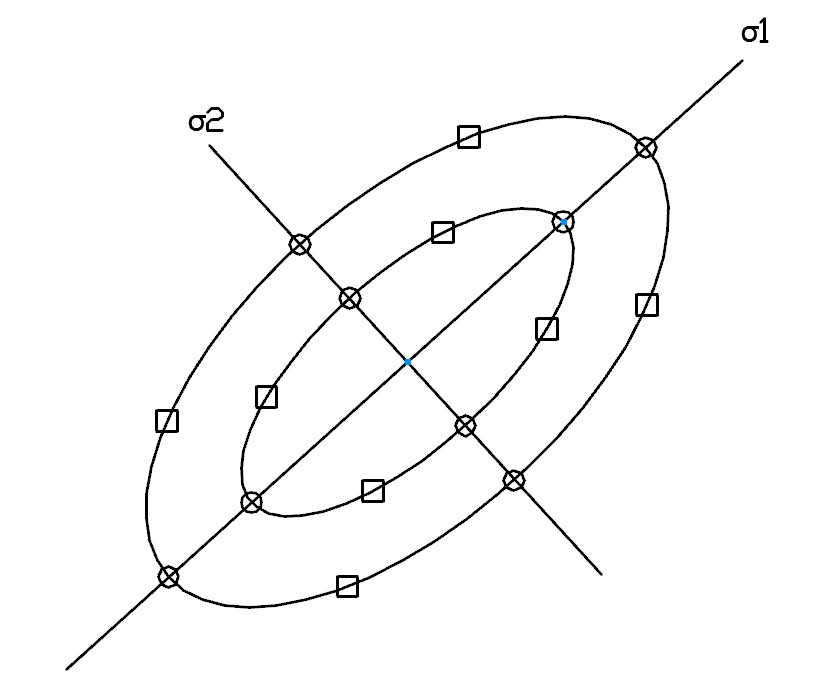
\includegraphics[width=0.3\textwidth]{4n1contours.jpg}
	\caption{4n+1 points on sigma contours}
	\label{fig:4np1pts}
\end{figure}\newline
 %******************
 There are two sets of points on each sigma contour. This is just to illustrate the diffenrene between the points derived from principle square root and cholesky decomposition of P. Cholesky decomposition results in points that lie on the ellipse/ contour but not on the principle axis. The points derived from the principle square root lie on the axis of the ellipse and the contour. 
 The mean and all higher order odd moments are automatically satisfied as the points are chosen to be symmetric. The covariance equations i.e. the second moments computed from the set of points (\ref{eq:points1}) are
\begin{align*} 
E[x_1^2]&=\sum{w_ix_{1i}^2}=(2w_1r_1^2+2w_2r_2^2)(\sigma_{11}^2+\sigma_{12}^2)=(2w_1r_1^2+2w_2r_2^2)P_{11}\\ E[x_1x_2]&=\sum{w_ix_{1i}x_{2i}}=(2w_1r_1^2+2w_2r_2^2)(\sigma_{11}\sigma_{12}+\sigma_{12}\sigma_{22})=(2w_1r_1^2+2w_2r_2^2)P_{12}\\
E[x_2^2]&=\sum{w_ix_{2i}^2}=(2w_1r_1^2+2w_2r_2^2)(\sigma_{12}^2+\sigma_{22}^2)=(2w_1r_1^2+2w_2r_2^2)P_{22}
 \end{align*} 
 Where we have used equations (\ref{eq:pp1})-(\ref{eq:pp2}).It can be seen that by choosing points on the sigma contours the 3 equations for a 2D case collapse into just solving one equations i.e.
 \begin{align}
 2w_1r_1^2+2w_2r_2^2&=1
 \end{align}
 Now looking at the 4th moment.
 \begin{align*} E[x_1^4]&=\sum{w_ix_{1i}^4}=(2w_1r_1^4+2w_2r_2^4)(\sigma_{11}^4+\sigma_{12}^4)\equiv 3P_{11}^2\\ E[x_1^3x_2]&=\sum{w_ix_{1i}^3x_{2i}^2}=(2w_1r_1^4+2w_2r_2^4)(\sigma_{11}^3\sigma_{12}+\sigma_{12}^3\sigma_{22})\equiv3P_{11}P_{12}\\
E[x_1^2x_2]&=\sum{w_ix_{1i}^2x_{2i}^2}=(2w_1r_1^4+2w_2r_2^4)(\sigma_{11}^2\sigma_{12}^2+\sigma_{12}^2\sigma_{22}^2)\equiv P_{11}P_{22}+2P_{12}^2\\
E[x_1^1x_2^3]&=\sum{w_ix_{1i}x_{2i}^3}=(2w_1r_1^4+2w_2r_2^4)(\sigma_{11}\sigma_{12}^3+\sigma_{12}\sigma_{22}^3)\equiv 3P_{22}P_{12}\\
E[x_2^4]&=\sum{w_ix_{2i}^4}=(2w_1r_1^4+2w_2r_2^4)(\sigma_{12}^4+\sigma_{22}^4)\equiv 3P_{22}^2\\ 
 \end{align*}
Here we have 5 equations which seem to have the same left hand side of variables $2w_1r_1^4+2w_2r_2^4$ but different right hand side of constant values. These are like parallel curves that do not intersect and cannot be solved for. It does not matter how many points we take on the principle axis or in general sigma contour formed from $\sqrt{P}$, we always end up in the above structure. But one may make a very nice inference that by choosing points on the sigma contours we can exactly match the mean and covariance.This gives us a clue that we need to search in some other direction in addition to principle axis for these sigma points.\newline\newline
{\bf Searching for Sigma points on principle axis and "conjugate axis" that can satisfy the 4th moment "`exactly"}\newline
	The term conjugate axis is just a name we chose to designate a particular axis of the ellipsoid and should not be confused with its meaning elsewhere. Again for a 2D case, the axis are chosen as\newline
	Principle axis:
\[\sigma_1=\left[ {\begin{array}{c}
 \sigma_{11}\\
 \sigma_{12}
 \end{array} } \right]\]
 \[\sigma_2=\left[ {\begin{array}{c}
 \sigma_{12}\\
 \sigma_{22}
 \end{array} } \right]\]
 Conjugate axis:
 \begin{align}
 \sigma_3=\sigma_1+\sigma_2\\
 \sigma_4=\sigma_1-\sigma_2
 \end{align}
 The points $(x_{1i},x_{2i})$ are therefore
  \begin{align*}
 &(0,0)\\
 &(r_1\sigma_{11},r_1\sigma_{12})\\
 &(-r_1\sigma_{11},-r_1\sigma_{12})\\
 &(r_1\sigma_{12},r_1\sigma_{22})\\
 &(-r_1\sigma_{12},-r_1\sigma_{22})\\
 &(r_2(\sigma_{11}+\sigma_{12}),r_2(\sigma_{12}+\sigma_{22}))\\
 &(-r_2(\sigma_{11}+\sigma_{12}),-r_2(\sigma_{12}+\sigma_{22}))\\
 &(r_2(\sigma_{11}-\sigma_{12}),r_2(\sigma_{12}-\sigma_{22}))
  \end{align*}
  \begin{equation}
 (-r_2(\sigma_{11}-\sigma_{12}),-r_2(\sigma_{12}-\sigma_{22}))\label{eq:points2}
\end{equation}
 Visually they look like \newline\newline
 %******************
\begin{figure}[h]
  \centering
	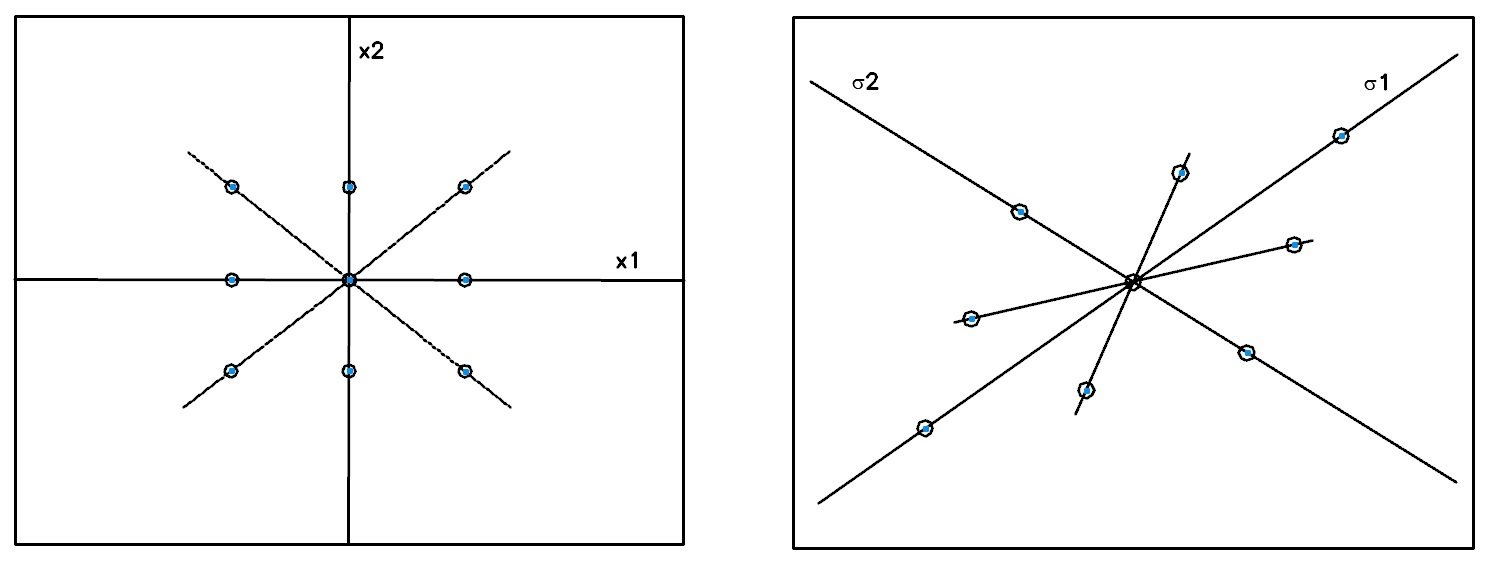
\includegraphics[width=0.7\textwidth]{2d4thmom.jpg}
	\caption{(a)Indentity Cov and (b)$[4,2;2,3]$ Cov}
	\label{fig:eye2quadpts}
\end{figure}\newline
 %******************
 Any arbitrary moment of a Gaussian PDF is given by {\bf Isserlis Theorem}:
 \begin{align}
 E[x_1x_2x_3....x_{2n}]=\sum\prod{E[x_ix_j]}
 \end{align} 
 for example the fourth moment is
 \begin{align}
 E[x_1x_2x_3x_4]&=E[x_1x_2]E[x_3x_4]+E[x_1x_3]E[x_4x_5]+E[x_1x_4]E[x_2x_3]
 \end{align}
 And the sixth moment is
 \begin{align*}
 E[x_1x_2x_3x_4x_5x_6]&=E[x_1x_2]E[x_3x_4]E[x_5x_6]    +E[x_1x_2]E[x_3x_5]E[x_4x_6]		+E[x_1x_2]E[x_3x_6]E[x_4x_5]\\
 &+E[x_1x_3]E[x_2x_4]E[x_5x_6]    +E[x_1x_3]E[x_2x_5]E[x_4x_6]		+E[x_1x_3]E[x_2x_6]E[x_4x_5]\\
 &+E[x_1x_4]E[x_2x_3]E[x_5x_6]		+E[x_1x_4]E[x_2x_5]E[x_3x_6]		+E[x_1x_4]E[x_2x_6]E[x_3x_5]\\
 &+E[x_1x_5]E[x_2x_3]E[x_4x_6]		+E[x_1x_5]E[x_2x_4]E[x_3x_6]		+E[x_1x_5]E[x_2x_6]E[x_3x_4]\\
 &+E[x_1x_6]E[x_2x_3]E[x_4x_5]		+E[x_1x_6]E[x_2x_4]E[x_3x_5]		+E[x_1x_6]E[x_2x_5]E[x_3x_4]
 \end{align*}
 The 2nd moment equations using the points set (\ref{eq:points2}) are
 \begin{align} E[x_1^2]&=\sum{w_ix_{1i}^2}=(2w_1r_1^2+4w_2r_2^2)(\sigma_{11}^2+\sigma_{12}^2)=(2w_1r_1^2+4w_2r_2^2)P_{11}\\ E[x_1x_2]&=\sum{w_ix_{1i}x_{2i}}=(2w_1r_1^2+4w_2r_2^2)(\sigma_{11}\sigma_{12}+\sigma_{12}\sigma_{22})=(2w_1r_1^2+4w_2r_2^2)P_{12}\\
E[x_2^2]&=\sum{w_ix_{2i}^2}=(2w_1r_1^2+4w_2r_2^2)(\sigma_{12}^2+\sigma_{22}^2)=(2w_1r_1^2+4w_2r_2^2)P_{22}
 \end{align} 
  Again by using equations (\ref{eq:pp1})-(\ref{eq:pp2}),from these 3 equations we are only left to solve the equation
 \begin{align}
 2w_1r_1^2+4w_2r_2^2&=1
 \end{align}
 Now if we consider the 5 - 4th order moments for the 2D case: \newline\newline
 for continuous system
 \begin{align*}
 E[x_1^4]&=3 P_{11}^2=3 (\sigma_{11}^4 + \sigma_{12}^4) + 6 (\sigma_{11}^2 \sigma_{12}^2)\\
 E[x_1^3x_2]&=3 P_{11} P_{12}=3 (\sigma_{11}^3 \sigma_{12}+ \sigma_{12}^3 \sigma_{22}) + 3( \sigma_{11} \sigma_{12}^3 +  \sigma_{11}^2 \sigma_{12} \sigma_{22}) \\
 E[x_1^2x_2]&=P_{11} P_{22} + 2 P_{12}^2=3 (\sigma_{11}^2 \sigma_{12}^2+ \sigma_{12}^2 \sigma_{22}^2  ) + (\sigma_{12}^4 + 4 \sigma_{11} \sigma_{12}^2 \sigma_{22} + \sigma_{11}^2 \sigma_{22}^2) \\
 E[x_1^1x_2^3]&=3 P_{22} P_{12}=3 (\sigma_{11} \sigma_{12}^3+  \sigma_{12} \sigma_{22}^3) + 3( \sigma_{12}^3 \sigma_{22} +  \sigma_{11} \sigma_{12} \sigma_{22}^2) \\
 E[x_2^4]&=3 P_{22}^2=3 (\sigma_{12}^4+  \sigma_{22}^4 )+ 6 (\sigma_{12}^2 \sigma_{22}^2 )
 \end{align*}
 For the equivalent discrete system the 4th order moments are
 \begin{align*}
E[x_1^4]&=\sum{w_ix_{1i}^4}=(\sigma_{11}^4+\sigma_{12}^4)(2 r_1^4 w_1 + 4 r_2^4 w_2)+24 w_2 r_2^4 (\sigma_{11}^2 \sigma_{12}^2)\\
E[x_1^3x_2]&=\sum{w_ix_{1i}^3x_{2i}^2}=(\sigma_{11}^3 \sigma_{12}+ \sigma_{12}^3 \sigma_{22})(2 r_1^4 w_1 + 4 r_2^4 w_2)+12 w_2 r_2^4(\sigma_{11} \sigma_{12}^3  + \sigma_{11}^2 \sigma_{12} \sigma_{22}) \\
E[x_1^2x_2]&=\sum{w_ix_{1i}^2x_{2i}^2}=(\sigma_{11}^2 \sigma_{12}^2+ \sigma_{12}^2 \sigma_{22}^2) (2 r_1^4 w_1 + 4 r_2^4 w_2)+4 w_2 r_2^4 (\sigma_{12}^4  + 4 \sigma_{11} \sigma_{12}^2 \sigma_{22} + \sigma_{11}^2 \sigma_{22}^2)  \\
E[x_1^1x_2^3]&=\sum{w_ix_{1i}x_{2i}^3}=(\sigma_{11} \sigma_{12}^3+\sigma_{12} \sigma_{22}^3) (2 r_1^4 w_1 + 4 r_2^4 w_2)+12 w_2 r_2^4(\sigma_{12}^3 \sigma_{22}  + \sigma_{11} \sigma_{12} \sigma_{22}^2)   \\
E[x_2^4]&=\sum{w_ix_{2i}^4}=(\sigma_{12}^4+\sigma_{22}^4)(2 r_1^4 w_1 + 4 r_2^4 w_2)+24 w_2 r_2^4 (\sigma_{12}^2 \sigma_{22}^2 )\\ 
 \end{align*}
 On comparing the set of equations for the continuous and discrete case, we are only left to solve the 2 equations
  \begin{align}
 2w_1r_1^4+4w_2r_2^4&=3\\
 4w_2r_2^4&=1
 \end{align}
 Now if we apply the same procedure to n-dimensional system we can generalise the set of equations. In summary 
 \begin{align}
 2w_1r_1^2+2^nw_2r_2^2&=1\\
  2w_1r_1^4+2^nw_2r_2^4&=3\\
 2^nw_2r_2^4&=1
 \end{align}
 The central weight at the mean is found by
 \begin{align}
 w_0&=1-2nw_1-2^nw_2
 \end{align}
 These equations have to be solved for $w_1,r_1,w_2,r_2$. In total there are $2n+2^n+1$ points.1 point of weight $w_0$ on the mean, $2n$ points of weight $w_1$ lie on the principle axis on the $r1\sqrt{P}$ contour, rest $2^n$ points lie on the conjugate axis symmetrically. \newline\newline
{\bf Results of integration compared to Gauss Hermite integration for 3D system}\newline\newline
Here in this section the new set of sigma points for 3D case are put to test, compared to gauss hermite integration. As the new set of points are only good till fourth moment we would consider the integration of polynomials till degree 4.\newline
\[
 P = \begin{bmatrix}
       4 & 2 & 1    \\
       2 & 9 & 1     \\
       1 & 1 & 16
     \end{bmatrix}
\]
\begin{align}
X&=[x_1,x_2,x_3]\\
F(X)&=x_1^4+x_2^4+x_3^4+x_1^3x_2+x_1^2x_2^2+\\
 &+x_3^2x_2^2+x_1^2x_3^2+x_1^3x_3+x_2^3x_3+x_3^3x_2
\end{align}
\begin{equation}
f=\int{F(X)N(X,0|P)}dX
\end{equation}
\begin{center}
  \begin{tabular}{ | l | l | l | l | l | }
    \hline
       No. of pts 					& $2^3=$ 8 							& $3^3=$ 27 			  & $4^3=$ 64			 & $10^3=$ 1000 (Truth) \\ \hline 
      GH          					&   1056.95571  			  & 1797.9999999      & 1798.00     	 &   1798.00           \\ \hline
\% error wrt Truth       	  &   41.2149211    			&  4.299e-013  	  	& 3.03502e-013   &   0         \\ 
      \hline
  \end{tabular}
\end{center} 

\begin{center}
  \begin{tabular}{ | l | l | l | l | l | }
    \hline
                  					&   No. of pts			& Integration result 			  & \% error wrt Truth			 \\ \hline 
      NM          					&   15       			  & 1797.99999998858          & 6.355208041935254e-010   \\
      \hline
  \end{tabular}
\end{center}
%*********************************************************************
{\bf Transformation of an arbitrary Jointly distributed Gaussian PDF into an i.i.d Gaussian PDF with mean zero }\newline\newline
	Any jointly distributed gaussian PDF can be transformed into a Gaussian PDF of zero mean and identity covariance of same dimension. This way one could find the sigma points in the i.i.d space and then transform each point into the original jointly distributed space. Firstly translate the jointly distributed pdf so that the mean coincides with origin. Then the transformation or here a scaled rotation is performed. The inverse of covariance matrix is expanded using a singular value decomposition.
	\begin{align}
	x^TP^{-1}x&=x^TU^T\Sigma Ux =x^TU^T\sqrt{\Sigma}\sqrt{\Sigma} Ux 
	\end{align}
	Let
	\begin{align}
	y=\sqrt{\Sigma}Ux
	\end{align}
	then
	\begin{align}
	x^TP^{-1}x&=y^Ty 
	\end{align}
	  Thus by the transformation $y=\sqrt{\Sigma}Ux$ we have the two Gaussian PDFs equivalent
	  \begin{align}
	  N(x,0|P)&\equiv N(y,0|I)
	  \end{align}
	  It is much easier to work with the i.i.d. gaussian variables. All the moments are preserved under this transformation. The principle axes just become
	  \begin{align}
	  \sigma_i=I_i
	  \end{align}
	  where I is the identity matrix of appropriate dimension and $I_i$ is the $i^{th}$ column of the I.
\newline\newline
{\bf Sigma points to capture the 6th moment exactly }\newline\newline
To capture the 6th order moments exactly extra points are taken on different set of axis. For example consider the 3D case. There are 3 principle axis $\sigma_1$, $\sigma_2$ and $\sigma_3$.Considering the mean to be the origin additional axis are constructed from these axis. \newline\newline
The 3 principle axis have 6 points. Each point is scaled with factor $r_1$ along the principle axis and has weight $w_1$
 \begin{align}
 \pm \sigma_1\nonumber\\
 \pm\sigma_2\nonumber\\
 \pm\sigma_3
 \end{align}
The conjugate axis have 8 points. Each point on this axis is scaled by $r_2$ and has weight $w_2$ 
\begin{align}
\pm\sigma_1\pm\sigma_2\pm\sigma_3
\end{align}
A new set of axis  are formed that lie in each of the orthogonal planes, they pass through the origin and are $45^o$ to each principle axis in that plane. The points are scaled by $r_3$ and have weight $w_3$. There are 12 pts on these axis
\begin{align}
\pm\sigma_1\pm\sigma_2 \nonumber\\
\pm\sigma_1\pm\sigma_3 \nonumber\\
\pm\sigma_2\pm\sigma_3
\end{align}
 In total there are $6+8+12=26$ sigma points to capture all the 6th order and lower moments for this 3D case.
 To intuitively realize the complete distribution in Figure (\ref{fig:3d1}) for 3D system  is difficult so the points only in one of the eight quadrants are shown in Figure (\ref{fig:3d2}). For 2D system there is more that one way where we can easily rearrange the points to capture the 6th moment. These two configurations are shown in figure (\ref{fig:2dconfigs}).\newline
%*******************
\begin{figure}[h]
	\centering
		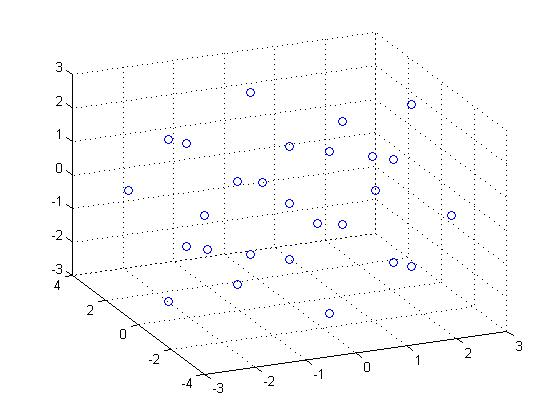
\includegraphics[width=0.40\textwidth]{3d6thmomentpts.jpg}
	\caption{Identity Cov 3D pts}
	\label{fig:3d1}
\end{figure}
\begin{figure}[h]
	\centering
		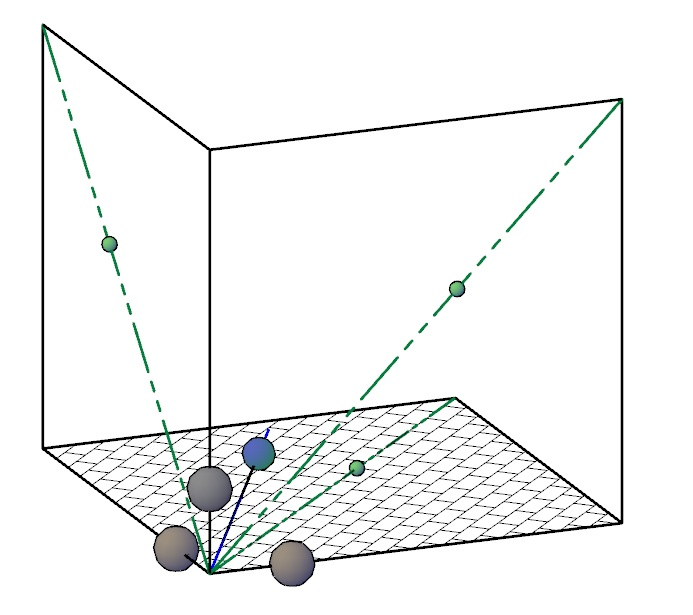
\includegraphics[width=0.35\textwidth]{3d6thmom.jpg}
	  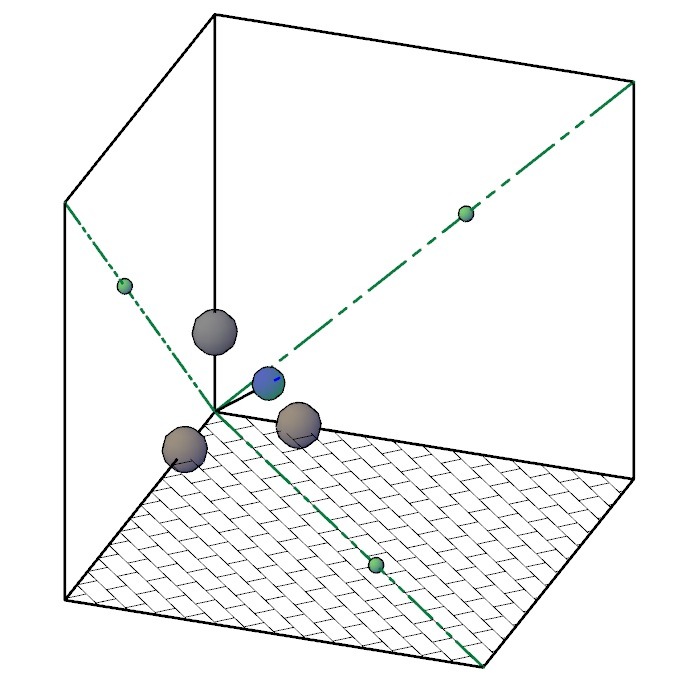
\includegraphics[width=0.325\textwidth]{3d6thmom2.jpg}
	\caption{Two perspective views of points in 1st quadrant of 3D space}
	\label{fig:3d2}
\end{figure}
 %******************
\begin{figure}[h]
	\centering
	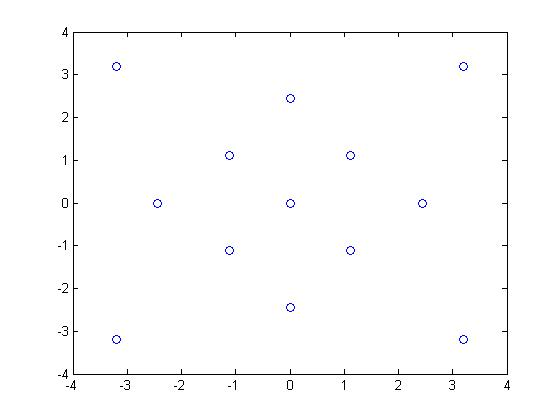
\includegraphics[width=0.4\textwidth]{2dcorr6thmomentpts.jpg}
	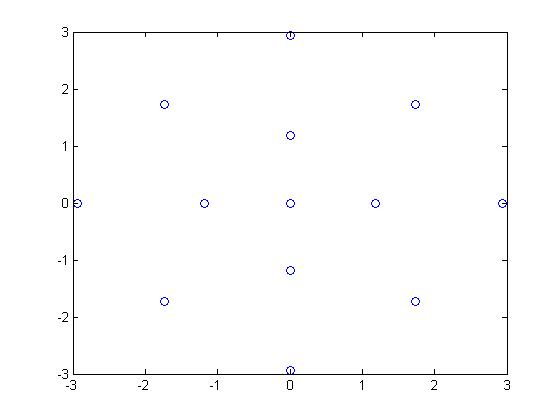
\includegraphics[width=0.4\textwidth]{2d_weird_case2.jpg}
	\caption{2 different configurations for 2D system}
	\label{fig:2dconfigs}
\end{figure}
 %******************
 For a general n- Dimensional system the equations to be solved a
 \begin{align*}
 2r_1^2w_1+2^nr_2^2w_2+4(n-1)r_3^2w_3&=1\\
 2r_1^4w_1+2^nr_2^4w_2+4(n-1)r_3^4w_3&=3\\
 2^nr_2^4w_2+4r_3^4w_3&=1\\
 2r_1^6w_1+2^nr_2^6w_2+4(n-1)r_3^6w_3&=15\\
 2^nr_2^6w_2+4r_3^6w_3&=3\\
 2^nr_2^6w_2&=1
 \end{align*}\newline\newline\newline
 {\bf Results of integration compared to Gauss Hermite integration for 4D system}\newline\newline
Here in this section the new set of sigma points to capture the 6th moment also for 4D case are put to test, compared to gauss hermite integration. As the new set of points are only good till sixth order moment we would consider the integration of polynomials till degree 6.\newline
 The covariance of the gaussian Kernel
\[
 P = \begin{bmatrix}
       4 & 1 & 2  & 1   \\
       1 & 9 & 2  & 3   \\
       2 & 2 & 16 & 4  \\
       1 & 3 & 4 & 25  
     \end{bmatrix}
\]
\begin{align}
X&=[x_1,x_2,x_3,x_4]\\
F(X)&=x_1^6+x_2^6+x_3^6+x_4^6+x_1^4+x_2^4+x_3^4+x_4^4+x_1^2x_2^2x_3^2+\nonumber\\
&+x_1^3x_3+x_1^2x_2^4+x_3^4x_2^2+x_1^2x_3^4+x_1^3x_3+x_2^3x_3+x_3^3x_2
\end{align}
Evaluating the integral
\begin{equation}
f=\int{F(X)N(X,0|P)}dX
\end{equation}
\begin{center}
  \begin{tabular}{ | l | l | l | l | l | l | }
    \hline
       No. of pts 					& $2^4=$ 16 							& $3^4=$ 81 			  & $4^4=$ 256			 & $5^4=$ 64 	  	& $20^4=$ 160000 (Truth) \\ \hline 
      GH          					&   84462.6354  		& 293311.8446    & 375417.9999     	 & 375417.9999  		  &   375417.9999           \\ \hline
\% error        	  &   77.5017    		&  21.8705  	  	& 9.0702e-012   & 8.9152e-012   &   0                      \\ 
      \hline 
  \end{tabular}
\end{center} 

\begin{center}
  \begin{tabular}{ | l | l | l | l | l | }
    \hline
                  					&   No. of pts			& Integration result 			  & \% error wrt Truth			 \\ \hline 
      NM          					&   49       			  & 3.754206e+005          & 7.112483626542660e-004   \\
      \hline
  \end{tabular}
\end{center}
%*****************************************************************
{\bf Sigma points to capture the 8th moment exactly }
To capture the 8th order moments exactly additional axis have to be considered. For example consider the 4D case. There are 4 principle axis $\sigma_1$, $\sigma_2$, $\sigma_3$ and $\sigma_4$. Additional axis constructed from these axis in the following way\newline\newline
The principle axis have 8 points with distance scaling factor $r_1$ and weight $w_1$
 \begin{align}
 \sigma_1 \nonumber \\
 \sigma_2 \nonumber \\
 \sigma_3 \nonumber \\
 \sigma_4
 \end{align}
The $2^{nd}$ set of axis are formed from considering all combinations of the principle axis. The disnce of each point is scaled by $r_2$ and each has weight $w_2$.
\begin{align}
\sigma_1 \pm \sigma_2 \pm \sigma_3 \pm \sigma_4
\end{align}
The $3^{rd}$ set of axis are constructed from considering 3 principle axis at a time. The corresponding distance scaling factor and weight are $r_5$ an $w_5$
\begin{align}
\sigma_1 \pm \sigma_2 \pm \sigma_3 \nonumber \\
\sigma_1 \pm \sigma_2 \pm \sigma_4 \nonumber \\
\sigma_1 \pm \sigma_3 \pm \sigma_4 \nonumber \\
\sigma_2 \pm \sigma_3 \pm \sigma_4 
\end{align}
The $4^{th}$ set of axis are constructed from considering 2 principle axis at a time. The corresponding distance scaling factor and weight are $r_3$ an $w_3$
\begin{align}
\sigma_1 \pm \sigma_2 \nonumber \\
\sigma_1 \pm \sigma_3 \nonumber \\
\sigma_1 \pm \sigma_4 \nonumber \\
\sigma_2 \pm \sigma_3 \nonumber \\
\sigma_2 \pm \sigma_4 \nonumber \\
\sigma_3 \pm \sigma_4 \nonumber 
\end{align}
The $5^{th}$ set of axis are fromed from considering all combinations of principle axis with one axis in each combination scaled with a parameter. The corresponding distance scaling factor and weight are $r_6$ an $w_6$ 
\begin{align}
 h \sigma_1 \pm \sigma_2 \pm \sigma_3 \pm \sigma_4 \nonumber \\
   \sigma_1 \pm h\sigma_2 \pm \sigma_3 \pm \sigma_4 \nonumber \\
   \sigma_1 \pm \sigma_2 \pm h\sigma_3 \pm \sigma_4 \nonumber \\
   \sigma_1 \pm \sigma_2 \pm \sigma_3 \pm h\sigma_4 \nonumber 
\end{align}
where h is the scaling parameter. When the scaling paramter $h=1$ then these set of axis match the $2^{nd}$ set of axis . As h slowly changes from 1 the axis start to diverge away from the $2^{nd}$ set of axis, but they are still arranged in space such that they are symmetrical. This additional set of axis can be visuallised for the 2D system in figure (\ref{fig:eye2quadpts}) and for 3D system in figure (\ref{fig:eye3quadpts}). Only one of the 8 quadrants of the 3D system is shown in different perspectives. All the quadrants are similar and symmetric abount mean.\newline
%********************************************************************
\begin{figure}[h]
	\centering
	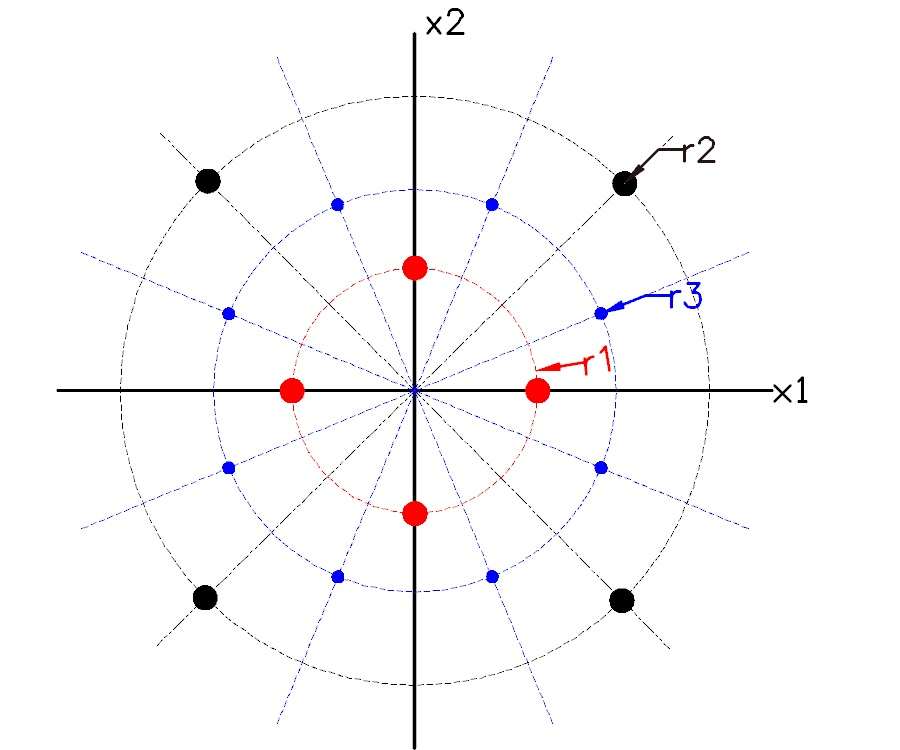
\includegraphics[width=0.5\textwidth]{2d1.jpg}
	\caption{2D system with points to capture 8th moment}
	\label{fig:eye2quadpts}
\end{figure}\newline
\begin{figure}[h]
	\centering
	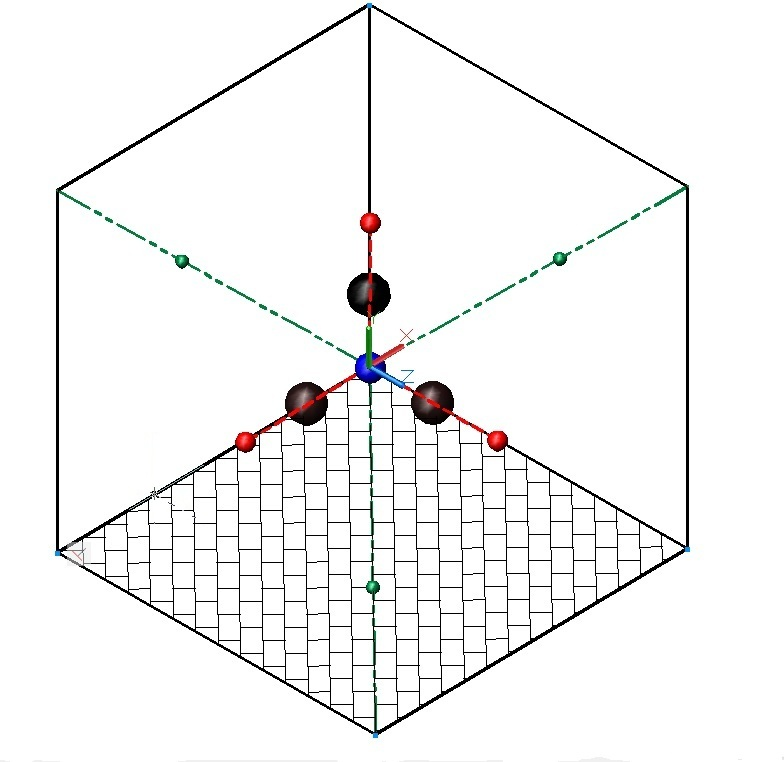
\includegraphics[width=0.3\textwidth]{3d2.jpg}
	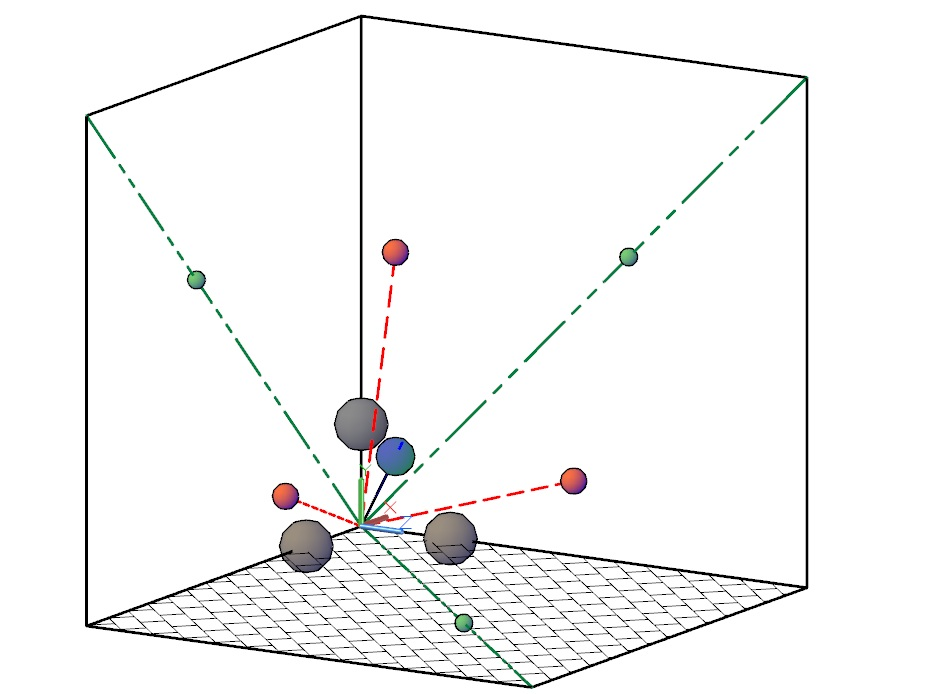
\includegraphics[width=0.35\textwidth]{3d3.jpg}
	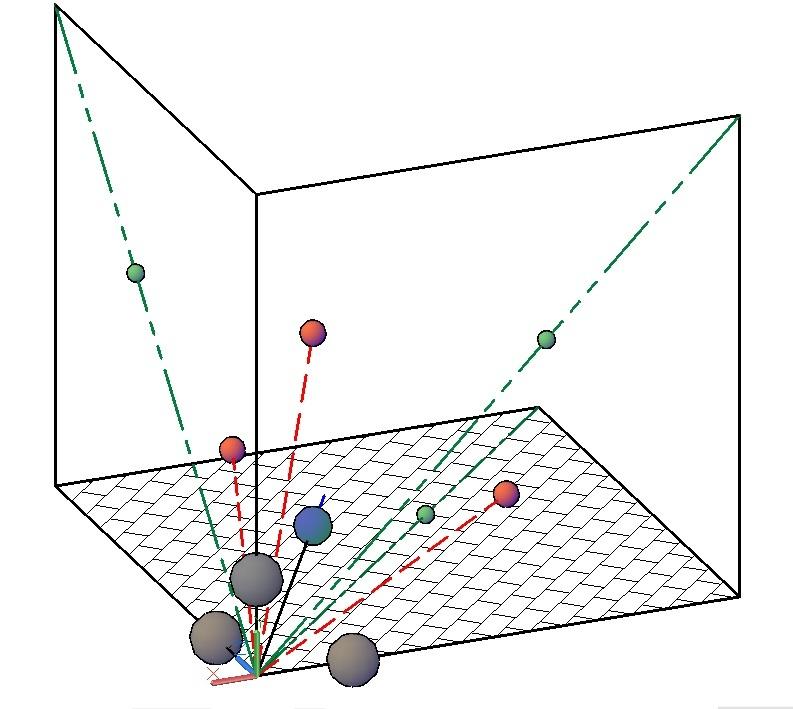
\includegraphics[width=0.3\textwidth]{3d4.jpg}
	\caption{1st quadrant of 3D system showing the points on axes}
	\label{fig:eye3quadpts}
\end{figure}
%**************************************************************
\newline This set of axis are very crucial to capture the various moments within the $8th$ set of moment. All the set of 8th moments are captured only when the points are situated in space, planar points cannot capture all the 8th moments. There are a total of 11 distinct equations in all from 2nd to 8th moment for sytems of dimension 4 or hihger. We thus need 11 variables to solve for. But by considering only the 5 set of axis above there will be only 10 variables in all $r_1,w_1,r_2,w_2,r_3,w_3,r_4,w_4,r_5,w_5$. Another set of points $r_4$ and weight $w_4$ are taken on the $2^nd$ set of axis : 12 variables and 11 equations to solve. We are free to choose the scaling parameter h and any one variable, or we could frame an optimization problem to minimize the error in the $10^{th}$ moment. The 11 equations to solve are
\begin{align*}
2r_1^2w_1+16r_2^2w_2+12r_3^2w_3+16r_4^2w_4+24r_5^2w_5+48r_6^2w_6+16h^2r_6^2w_6&=1\\
2r_1^4w_1+16r_2^4w_2+12r_3^4w_3+16r_4^4w_4+24r_5^4w_5+48r_6^4w_6+16h^4r_6^4w_6&=3\\
16r_2^4w_2+4r_3^4w_3+16r_4^4w_4+16r_5^4w_5+32r_6^4w_6+32h^2r_6^4w_6&=1\\
2r_1^6w_1+16r_2^6w_2+12r_3^6w_3+16r_4^6w_4+24r_5^6w_5+48r_6^6w_6+16h^6r_6^6w_6&=15\\
16r_2^6w_2+4r_3^6w_3+16r_4^6w_4+16r_5^6w_5+32r_6^6w_6+16h^2r_6^6w_6+16h^4r_6^6w_6&=3\\
16r_2^6w_2+16r_4^6w_4+8r_5^6w_5+16r_6^6w_6+48h^2r_6^6w_6&=1\\
2r_1^8w_1+16r_2^8w_2+12r_3^8w_3+16r_4^8w_4+24r_5^8w_5+48r_6^8w_6+16h^8r_6^8w_6&=105\\
16r_2^8w_2+4r_3^8w_3+16r_4^8w_4+16r_5^8w_5+32r_6^8w_6+16h^2r_6^8w_6+16h^6r_6^8w_6&=15\\
16r_2^8w_2+4r_3^8w_3+16r_4^8w_4+16r_5^8w_5+32r_6^8w_6+32h^4r_6^8w_6&=9\\
16r_2^8w_2+16r_4^8w_4+8r_5^8w_5+16r_6^8w_6+32h^2r_6^8w_6+16h^4r_6^8w_6&=3\\
16r_2^8w_2+16r_4^8w_4+64h^2r_6^8w_6&=1\\
\end{align*}     

And similarly for a 5-D system the equations are
\begin{align*}
2r_1^2w_1+32r_2^2w_2+16r_3^2w_3+32r_4^2w_4+48r_5^2w_5+128r_6^2w_6+32h^2r_6^2w_6&=1\\
2r_1^4w_1+32r_2^4w_2+16r_3^4w_3+32r_4^4w_4+48r_5^4w_5+128r_6^4w_6+32h^4r_6^4w_6&=3\\
32r_2^4w_2+4r_3^4w_3+32r_4^4w_4+24r_5^4w_5+96r_6^4w_6+64h^2r_6^4w_6&=1\\
2r_1^6w_1+32r_2^6w_2+16r_3^6w_3+32r_4^6w_4+48r_5^6w_5+128r_6^6w_6+32h^6r_6^6w_6&=15\\
32r_2^6w_2+4r_3^6w_3+32r_4^6w_4+24r_5^6w_5+96r_6^6w_6+32h^2r_6^6w_6+32h^4r_6^6w_6&=3\\
32r_2^6w_2+32r_4^6w_4+8r_5^6w_5+64r_6^6w_6+96h^2r_6^6w_6&=1\\
2r_1^8w_1+32r_2^8w_2+16r_3^8w_3+32r_4^8w_4+48r_5^8w_5+128r_6^8w_6+32h^8r_6^8w_6&=105\\
32r_2^8w_2+4r_3^8w_3+32r_4^8w_4+24r_5^8w_5+96r_6^8w_6+32h^2r_6^8w_6+32h^6r_6^8w_6&=15\\
32r_2^8w_2+4r_3^8w_3+32r_4^8w_4+24r_5^8w_5+96r_6^8w_6+64h^4r_6^8w_6&=9\\
32r_2^8w_2+32r_4^8w_4+8r_5^8w_5+64r_6^8w_6+64h^2r_6^8w_6+32h^4r_6^8w_6&=3\\
32r_2^8w_2+32r_4^8w_4+32r_6^8w_6+128h^2r_6^8w_6&=1\\
\end{align*}
For a N-D system the total number of points required to capture the 8th moment  by this scheme are $1+2n^2+\frac{4n(n-1)(n-2)}{3}+(n+2)2^n$. A simple process of solving these equations is to first consider 6 equations preferably the last 6 of the 11 equations and to solve for the weights $w_1,w_2,w_3,w_4,w_5,w_6$ symbolically using Mathematica. Substitute these 6 weight equations into the remaining 5 equations. These 5 equations are now in terms of the distances $r_1,r_2,r_3,r_4,r_5,r_6$. One of the distance could be assumed a suitable value and the rest of the 5 equations can be solved for the remaining 5 varibles. An instance of the solution for the 5D system followed by this procedure, where $r_5$ and $h$ are assumed, is 
\begin{align}
h&=3 \nonumber \\
r_5&=2\nonumber\\
r_1&=2.3143708172807447\nonumber\\
r_2&=0.8390942773980102\nonumber\\
r_3&=1.8307521253266494\nonumber\\
r_4&=1.3970397430644959\nonumber\\
r_6&=1.1134786327367021\nonumber\\
w_1 &= 0.010529034221546607\nonumber\\
w_2 &= 0.015144019639537572\nonumber\\
w_3 &= 0.0052828996967816825\nonumber\\
w_4&=0.0010671298950159158\nonumber\\
w_5&=0.0006510416666666666\nonumber\\
w_6 &= 0.00013776017592074394 \label{eq:sol1}
\end{align}
 \newline\newline\newline\newline\newline\newline
 {\bf Results of integration compared to Gauss Hermite integration for 5D system}\newline\newline
The new set of sigma points are evaluated to capture the 8th moment in addition to all previous moments and all higher order odd moments. For 5-D case, the points are created along their respective axis with the distances and weights given in solution (\ref{eq:sol1}). These points are used to evaluate the integral and this result is compared to gauss hermite quadrature integration. As the new set of points are only good till 8th order moments we would consider the integration of ap olynomial till degree 8.\newline
 The covariance of the gaussian Kernel
\begin{align}
P=1000I_{5x5}
\end{align}
\begin{align}
X&=[x_1,x_2,x_3,x_4,x_5]\\
F(X)&=x_1^8+x_2^8+x_3^6+x_4^6+x_1^4x_5^4+x_2^4x_3^4+x_4^2+x_1^2x_2^2x_3^2x_4^2+\nonumber \\
&+x_1^3x_3+x_1^4x_2^2x_5^2+x_3^4x_2^2+x_1^2x_3^4+x_1^3x_3+x_2^3x_3+x_3^3x_2
\end{align}
Evaluating the integral
\begin{equation}
f=\int{F(X)N(X,0|P)}dX
\end{equation}
\begin{center}
  \begin{tabular}{ | l | l | l | l | l | l | }
    \hline
       No. of pts 					& $2^5=$ 32 				& $3^5=$ 243 			   & $4^5=$ 1024			   & $5^5=$ 3125  	    &  $15^5=$759375(Truth)                \\ \hline 
       GH          					& 6.0962801e+012 		& 7.6616634e+013     & 1.84964e+014      	 & 2.329646e+014  		  &   2.3296463e+014           \\ \hline
    \% error            	  & 97.38317      		&  67.11233  	    	 & 20.6039857          & 5.184531e-011       &   0                     \\ 
      \hline 
  \end{tabular}
\end{center} 

\begin{center}
  \begin{tabular}{ | l | l | l | l | l | }
    \hline
                  					&   No. of pts			& Integration result 			    & \% error wrt Truth			 \\ \hline 
      NM          					&   355       		  & 2.3296463e+014              & 5.1509964e-011   \\
      \hline
  \end{tabular}
\end{center}
The multi dimensional Gauss Hermite points amount to $3125$ to capture the 8th moment and lower order moments . It is evident that by the new set of sigma points we need only 355 points to attain the same order of accuracy as that of traditional gauss hermite quadrature with $3125$ points, while integrating polynomials of degree 8 or lower.
\end{document}  